\listoftodos

\chapter{Instance Segmentation: A brief look at the current state}
\label{chap:kapitel1}
- Instance Segmentation in general -> difficulties in this field (clutter/overlapping objects/Occlusion (you only can see small parts), novel objects -> CNN are not good in generalizing, challenging materials(Translucent, Reflective))
- Instance segmentaion is important-> examples
- Many data needed -> expensive
- Labeling expensive -> so often synthetic generation with a simuluation / a virtual environment are used and this is very promising
- 1. Through the gab of sim-to-real often depth images are used
- newer research suggest that rgb only can achieve even better results -> how can that be? What is now the real state of depth data for instance segmentation?
- There are many ways to use depth information (only D, RGBD, 2 pipelines, ...)
- 2. Often discussed is also the texture shape bias, which also seems to be a bit unclear -> and it cold be interesting to see it's influence with depth data -> thesis: texture + shape bias = good performance
- 3. there is not much research about the amount of shapes and materials -> the reason should be that it is very likely to see a better result/generalization with more textures and shapes. Neverless it could be interesting to see how much influence this have on the performance -> less shapes and textures can also lead to less expenses

 \cite{Fowler2014}.

	\section{Microservices}
	\label{sec:microservices}
	Lorem ipsum dolor sit amet, consetetur sadipscing elitr, sed diam nonumy eirmod tempor invidunt ut labore et dolore magna aliquyam erat, sed diam voluptua. At vero eos et accusam et justo duo dolores et ea rebum. Stet clita kasd gubergren, no sea takimata sanctus est Lorem ipsum dolor sit amet. Lorem ipsum dolor sit amet, consetetur sadipscing elitr, sed diam nonumy eirmod tempor invidunt ut labore et dolore magna aliquyam erat, sed diam voluptua. At vero eos et accusam et justo duo dolores et ea rebum. Stet clita kasd gubergren, no sea takimata sanctus est Lorem ipsum dolor sit amet. Referenz zur Abbildung \ref{img:microprofile}.
	\begin{figure}[h]
		\centering
		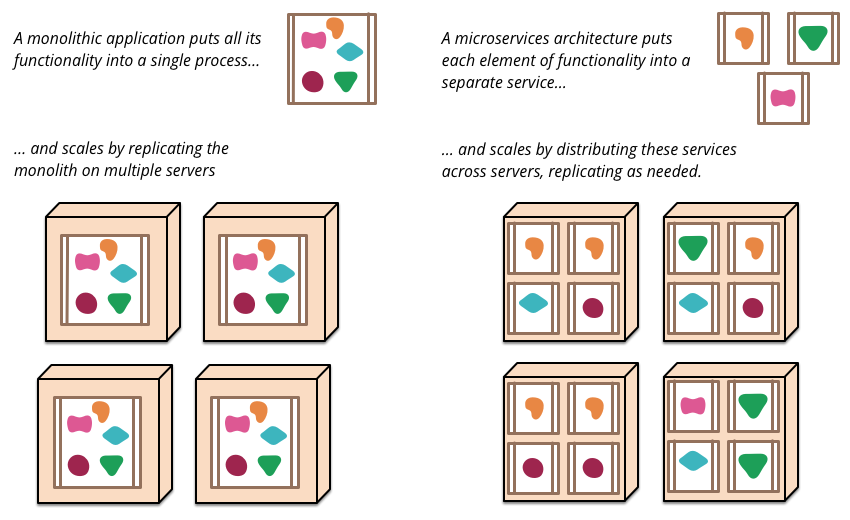
\includegraphics[width=\textwidth, center]{kapitel1/monolith_vs_microservices}
		\caption[Beschreibung für Verzeichnis]{Bildunterschrift}
		\label{img:microprofile}
	\end{figure}
	
	\subsection{Was sind Microservices}
	Lorem ipsum dolor sit amet, consetetur sadipscing elitr, sed diam nonumy eirmod tempor invidunt ut labore et dolore magna aliquyam erat, sed diam voluptua. At vero eos et accusam et justo duo dolores et ea rebum. Stet clita kasd gubergren, no sea takimata sanctus est Lorem ipsum dolor sit amet. Lorem ipsum dolor sit amet, consetetur sadipscing elitr, sed diam nonumy eirmod tempor invidunt ut labore et dolore magna aliquyam erat, sed diam voluptua. At vero eos et accusam et justo duo dolores et ea rebum. Stet clita kasd gubergren, no sea takimata sanctus est Lorem ipsum dolor sit amet \cite{Reese2009}.
	
	\paragraph{Klein und spezialisiert} Lorem ipsum dolor sit amet, consetetur sadipscing elitr, sed diam nonumy eirmod tempor invidunt ut labore et dolore magna aliquyam erat, sed diam voluptua. At vero eos et accusam et justo duo dolores et ea rebum. Stet clita kasd gubergren, no sea takimata sanctus est Lorem ipsum dolor sit amet. Lorem ipsum dolor sit amet, consetetur sadipscing elitr, sed diam nonumy eirmod tempor invidunt ut labore et dolore magna aliquyam erat, sed diam voluptua. At vero eos et accusam et justo duo dolores et ea rebum. Stet clita kasd gubergren, no sea takimata sanctus est Lorem ipsum dolor sit amet.
	
	\paragraph{Eigenständig} Lorem ipsum dolor sit amet, consetetur sadipscing elitr, sed diam nonumy eirmod tempor invidunt ut labore et dolore magna aliquyam erat, sed diam voluptua. At vero eos et accusam et justo duo dolores et ea rebum. Stet clita kasd gubergren, no sea takimata sanctus est Lorem ipsum dolor sit amet. Lorem ipsum dolor sit amet, consetetur sadipscing elitr, sed diam nonumy eirmod tempor invidunt ut labore et dolore magna aliquyam erat, sed diam voluptua. At vero eos et accusam et justo duo dolores et ea rebum. Stet clita kasd gubergren, no sea takimata sanctus est Lorem ipsum dolor sit amet. Verweis auf Anhang \ref{appendix:anhanga} \nameref{appendix:anhanga}
